% !Mode:: "TeX:UTF-8"
% Translator: Kai Li
\chapter{\gls{CNN}}
\label{chap:convolutional_networks}

\firstgls{convolutional_network}\citep{LeCun89a},也叫做\firstall{CNN},是一种专门用来处理具有类似网格结构的数据的神经网络。
例如时间序列数据(可以认为是在时间轴上有规律地采样形成的一维网格)和图像数据(可以看作是二维的像素网格)。
\gls{convolutional_network}在诸多应用领域都表现优异。
``\gls{convolutional_network}''一词表明该网络使用了\firstgls{convolution}这种数学运算。
卷积是一种特殊的线性运算。
\emph{\gls{convolutional_network}是指那些至少在网络的一层中使用卷积运算来替代一般的矩阵乘法运算的神经网络。}

本章,我们首先说明什么是卷积运算。
接着,我们会解释在神经网络中使用卷积运算的动机。
然后我们会介绍一种几乎所有的\gls{CNN}都会用到的操作\firstgls{pooling}。
通常来说,\gls{CNN}中用到的卷积运算和其他领域(例如工程领域以及纯数学领域)中的定义并不完全一致。
我们会对神经网络实践中用得比较多的几种卷积函数的变体进行说明。
我们也会说明如何在多种不同维数的数据上使用卷积运算。
之后我们讨论使得卷积运算更加高效的一些方法。
\gls{CNN}是神经科学的原理影响深度学习的典型代表,我们之后也会讨论这些神经科学的原理,并对卷积神经网路在深度学习发展史中的作用作出评价。
本章没有涉及如何为你的卷积神经网路选择合适的结构,因为本章的目标是说明\gls{CNN}提供的强大工具,第\ref{chap:practical_methodology}章会对在具体环境中使用相应的工具给出一些指导。
对于\gls{convolutional_network}结构的研究进展得如此迅速,以至于针对特定问题,数月甚至几周就会产生一个新的最优的网络结构,甚至在写这本书时也不好描述究竟哪种结构是最好的。
然而,最好的结构也是由本章所描述的基本部件一点一点搭建起来的。

% -- 321 --
 
\section{卷积运算}
\label{sec:the_convolution_operation}

在通常形式中,卷积是对两个实值函数的一种数学运算。
为了给出卷积的定义,我们从两个可能会用到的函数的例子出发。

假设我们正在用激光传感器追踪一艘宇宙飞船的位置。
我们的激光传感器给出一个单独的输出$x(t)$,表示宇宙飞船在时刻$t$ 的位置。
$x$和$t$都是实值的,这意味着我们可以在任意时刻从传感器中读出飞船的位置。

现在假设我们的传感器含有噪声。
为了得到飞船位置的低噪声估计,我们对得到的测量结果进行平均。
显然,时间上越近的测量结果越相关,所以我们采用一种加权平均的方法,对于最近的测量结果赋予更高的权值。
我们可以采用一个加权函数$w(a)$ 来实现,其中$a$表示测量结果据当前时刻的时间间隔。
如果我们对任意时刻都采用这种加权平均的操作,就得到了对于飞船位置的连续估计函数$s$:
\begin{equation}
s(t) = \int x(a)w(t-a)da.
\end{equation}

这种运算就叫做\firstgls{convolution}。
卷积运算通常用星号表示:
\begin{equation}
s(t) = (x*w)(t).
\end{equation}

在我们的例子中,$w$必须是一个有效的概率密度函数,否则输出就不再是一个加权平均。
另外,$w$在参数为负值时必须为0,否则它会涉及到未来,这不是我们能够做到的。
但这些限制仅仅是对我们这个例子来说。
通常,卷积被定义在满足上述积分式的任意函数上,并且也可能被用于加权平均以外的目的。

在\gls{CNN}的术语中,第一个参数(在这个例子中,函数$x$)叫做\firstgls{input},第二个参数(函数$w$)叫做\firstgls{kernel}。
输出有时被称作\firstgls{feature_map}。

% -- 322 --
 
在我们的例子中,激光传感器能够在任意时刻给出测量结果的想法是不现实的。
一般地,当我们用计算机处理数据时,时间会被离散化,传感器会给出特定时间间隔的数据。
所以比较现实的的假设是传感器每秒给出一次测量结果,这样,时间$t$只能取整数值。
如果我们假设$x$和$w$都定义在整数时刻$t$上,就得到了离散形式的卷积:
\begin{equation}
s(t) = (x*w)(t) = \sum_{a = -\infty}^{\infty} x(a)w(t-a).
\end{equation}

在机器学习的应用中,输入通常是高维数据数组,而核也是由算法产生的高维参数数组。
我们把这种高维数组叫做张量。
因为输入与核的每一个元素都分开存储,我们经常假设在存储了数据的有限点集以外,这些函数的值都为零。
这意味着在实际操作中,我们可以统一地把无限的求和当作对有限个数组元素的求和来用。

最后,我们有时对多个维度进行卷积运算。
例如,如果把二维的图像$I$作为输入,我们也相应的需要使用二维的核$K$:
\begin{equation}
S(i,j) = (I*K)(i,j) = \sum_m \sum_n I(m,n) K(i-m, j-n).
\end{equation}

卷积是可交换的,我们可以等价地写作:
\begin{equation}
S(i, j) = (K*I)(i,j) = \sum_m \sum_n I(i-m, j-n) K(m, n).
\end{equation}

通常,下面的公式在机器学习库中更方便应用,因为它在$m$和$n$的有效范围内变化更少。%(这是为什么?)

% -- 323 --
 
卷积运算可交换性的出现是因为我们相对输入\firstgls{flip}了核,这意味着当$m$增大时,输入的索引增大,但核的索引相应的减小。
翻转核的唯一目的就是为了得到可交换性。
尽管可交换性在证明时很有用,但在神经网络的应用中却不是一个重要的性质。
与之不同的是,许多神经网络库会实现一个相关的函数,称为\firstgls{cross_correlation},和卷积运算几乎一样但是并不翻转核:
\begin{equation}
S(i, j) = (I*K)(i, j) = \sum_m \sum_n I(i+m, j+n) K(m, n).
\end{equation}
许多机器学习的库使用互相关函数但是叫它卷积。
在这本书中我们遵循把两种运算都叫做卷积的这个传统,只有在用到核的翻转时才会在上下文中特别指明区别。
在机器学习中,学习算法会在核合适的位置学得恰当的值, 所以一个基于核翻转的卷积运算的学习算法所学得的核,是对未进行翻转的算法学得的核的翻转。
单独使用卷积运算在机器学习中是很少见的,卷积经常和其他的函数一起使用,无论卷积运算是否翻转了它的核,这些函数的组合通常是不可交换的。

图\ref{fig:chap9_conv_2d}演示了一个在二维张量上的卷积运算(核没有翻转)的例子。
% fig 9.1
\begin{figure}[!htb]
\ifOpenSource
\centerline{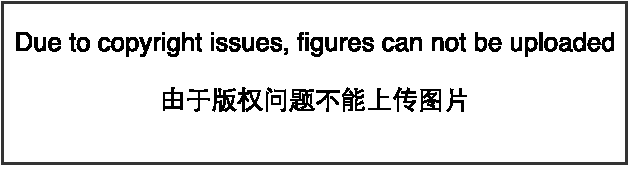
\includegraphics{figure.pdf}}
\else
\centerline{\includegraphics{Chapter9/figures/conv_2d}}
\fi
\caption{Tmp}
\label{fig:chap9_conv_2d}
\end{figure}

离散卷积可以看作矩阵的乘法,然而,这个矩阵的一些元素被限制为必须和另一些元素相等。
例如对于单变量的离散卷积,矩阵的每一行都必须和上一行移动一个元素后相等。
这种矩阵叫做\firstgls{Toeplitz_matrix}。
对于二维情况,卷积对应着一个\firstgls{doubly_block_circulant_matrix}。
除了这些元素相等的限制以外,卷积通常对应着一个非常稀疏的矩阵(几乎所有的元素都为零)。
这是因为核通常要远小于输入的图像。任何一个使用矩阵乘法但是并不依赖矩阵结构的特殊性质的神经网络算法,都适用于卷积运算,并且不需要对神经网络做出大的修改。
典型的\gls{CNN}为了更有效地处理大规模输入,确实使用了一些专门化的技巧,但这些在理论分析方面并不是严格必要的。

% -- 324 --
 
\section{动机}
\label{sec:motivation}

卷积运算通过三个重要的思想来帮助改进机器学习系统:\firstgls{sparse_interactions}、\firstgls{parameter_sharing}、\firstgls{equivariant_representations}。
另外,卷积提供了一种处理大小可变的输入的方法。
我们下面依次介绍这些思想。

传统的神经网络使用矩阵乘法来建立输入与输出的连接关系。
其中,参数矩阵的每一个独立的参数都描述了每一个输入单元与每一个输出单元间的交互。
这意味着每一个输出单元与每一个输入单元都产生交互。
然而,\gls{CNN}具有\firstgls{sparse_interactions}(也叫做\firstgls{sparse_connectivity}或者\firstgls{sparse_weights})的特征。
这通过使得核的规模远小于输入的规模来实现。
举个例子,当进行图像处理时,输入的图像可能包含百万个像素点,但是我们可以通过只占用几十到上百个像素点的核来探测一些小的有意义的特征,例如图像的边缘。
这意味着我们需要存储的参数更少,不仅减少了模型的存储需求,而且提高了它的统计效率。
这也意味着为了得到输出我们只需要更少的计算量。
这些效率上的提高往往是很显著的。
如果有$m$个输入和$n$个输出,那么矩阵乘法需要$m \times n$个参数并且相应算法的时间复杂度为$O(m\times n)$(对于每一个例子)。
如果我们限制每一个输出拥有的连接数为$k$,那么稀疏的连接方法只需要$k\times n$个参数以及$O(k\times n)$的运行时间。
在很多应用方面,只需保持$k$的数量级远小于$m$,就能在机器学习的任务中取得好的表现。
\gls{sparse_connectivity}的图形化解释如图\ref{fig:chap9_area_of_effect}和图\ref{fig:chap9_receptive_field}所示。
在深度\gls{convolutional_network}中,处在深层的单元可能\emph{不直接}地与绝大部分输入连接,如图\ref{fig:chap9_deep_receptive_field}所示。
这允许网络可以通过只描述\gls{sparse_interactions}的基石来高效地描述多个变量的复杂交互。
% fig 9.2
\begin{figure}[!htb]
\ifOpenSource
\centerline{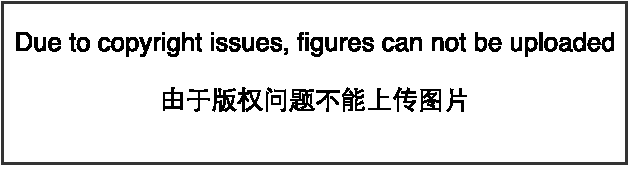
\includegraphics{figure.pdf}}
\else
\centerline{\includegraphics{Chapter9/figures/area_of_effect}}
\fi
\caption{Tmp}
\label{fig:chap9_area_of_effect}
\end{figure}
% fig 9.3
\begin{figure}[!htb]
\ifOpenSource
\centerline{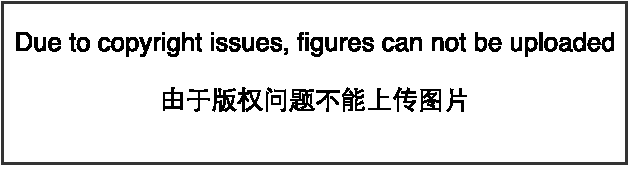
\includegraphics{figure.pdf}}
\else
\centerline{\includegraphics{Chapter9/figures/receptive_field}}
\fi
\caption{Tmp}
\label{fig:chap9_receptive_field}
\end{figure}
% fig 9.4
\begin{figure}[!htb]
\ifOpenSource
\centerline{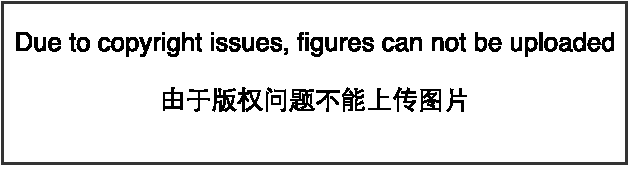
\includegraphics{figure.pdf}}
\else
\centerline{\includegraphics{Chapter9/figures/deep_receptive_field}}
\fi
\caption{Tmp}
\label{fig:chap9_deep_receptive_field}
\end{figure}

% -- 325 --
 
\firstgls{parameter_sharing}是指在一个模型的多个函数中使用相同的参数。
在传统的神经网络中,当计算一层的输出时,权值矩阵的每一个元素只使用一次,当它乘以输入的一个元素后就再也不会用到了。
作为\gls{parameter_sharing}的同义词,我们可以说一个网络含有\firstgls{tied_weights},因为一个用于输入的权值也被绑定在其他的权值上。
在\gls{CNN}中,核的每一个元素都作用在输入的每一位置上(除了一些可能的边界像素,取决于对于边界的决策设计)。
卷积运算中的\gls{parameter_sharing}保证了我们只需要学习一个参数集合,而不是对于每一位置都需要学习一个单独的参数集合。
这虽然没有改变前向传播的时间(仍然是$O(k\times n)$),但它显著地把模型的存储需求降低至$k$个参数,并且$k$通常是远小于$m$的数量级。
因为$m$ 和$n$通常很接近,$k$在实际中相对于$m\times n$是很小的。
因此,卷积在存储需求和统计效率方面极大地优于稠密矩阵的乘法运算。
图\ref{fig:chap9_parameter_sharing}演示了\gls{parameter_sharing}是如何实现的。
% fig 9.5
\begin{figure}[!htb]
\ifOpenSource
\centerline{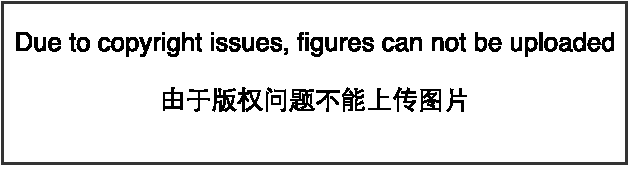
\includegraphics{figure.pdf}}
\else
\centerline{\includegraphics{Chapter9/figures/parameter_sharing}}
\fi
\caption{Tmp}
\label{fig:chap9_parameter_sharing}
\end{figure}
% -- 326 --
 
% -- 327 --
 
作为前两条原则的一个实际例子,图\ref{fig:chap9_efficiency_of_edge_detection}说明了\gls{sparse_connectivity}和\gls{parameter_sharing}是如何显著地提高图像中边缘检测的线性函数的效率的。
% fig 9.6
\begin{figure}
\ifOpenSource
\centerline{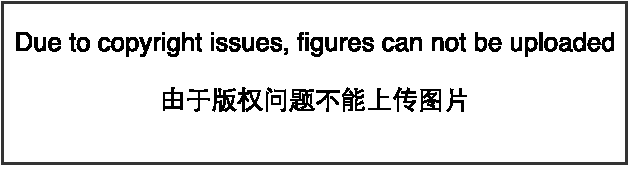
\includegraphics{figure.pdf}}
\else
\centering    
\subfigure{ \label{fig:chap9_efficiency_of_edge_detection_a}     
\includegraphics[width=0.35\textwidth]{Chapter9/figures/sundance.png}}     
\subfigure{ \label{fig:chap9_efficiency_of_edge_detection_b}     
\includegraphics[width=0.35\textwidth]{Chapter9/figures/edges.png}}     
\fi
\caption{Tmp}     
\label{fig:chap9_efficiency_of_edge_detection}     
\end{figure}
% -- 328 --
 
对于卷积,\gls{parameter_sharing}的特殊形式使得神经网络层具有对平移\firstgls{equivariance}的性质。
如果一个函数满足输入改变,输出也以同样的方式改变这一性质,我们就说它是等变(equivariant)的。
特别地,如果函数$f(x)$与$g(x)$满足$f(g(x))= g(f(x))$,我们就说$f(x)$对于变换$g$具有等变性。
对于卷积来说,如果令$g$是输入的任意平移函数,那么卷积函数对于$g$具有等变性。
举个例子,令$I$表示图像的明亮度函数(取值为整数),$g$表示图像函数的变换函数(把一个图像函数映射到另一个图像函数的函数)使得$I' = g(I)$,其中$I'(x,y) = I(x-1, y)$。
这个函数把$I$中的每个像素向右移动一格。
如果我们先对$I$进行变换然后进行卷积操作所得到的结果,与先对$I$进行卷积然后再对输出使用平移函数$g$得到的结果是一样的\footnote{译者注:原文将此处误写成了$I'$。} 。%译者注
当处理时间序列数据时,卷积产生一条用来表明输入中出现不同特征的某种时间轴。
如果我们把输入中的一个事件向后延时,在输出中也会有完全相同的表示,只是时间延时了。
图像与之类似,卷积产生了一个2维映射来表明某种属性在输入的什么位置出现了。
如果我们移动输入中的对象,它的表示也会在输出中移动同样的量。
当处理多个输入位置时,一些作用在邻居像素的函数是很有用的。
例如在处理图像时,在\gls{CNN}的第一层进行图像的边缘检测是很有用的。
相同的边缘或多或少地散落在图像的各处,所以应当对整个图像进行\gls{parameter_sharing}。
但在某些情况下,我们并不希望对整幅图进行\gls{parameter_sharing}。
例如当我们在处理人脸图像(图像已经被剪裁成人脸在中心)时,我们可能会希望在不同的部位探测出不同的特征(处理人脸上部的网络需要去搜寻眉毛,处理人脸下部的网络就需要去搜寻下巴了)。

% -- 329 --
 
卷积对其他的一些变换并不是天然等变的,例如对于图像尺度或者角度的变换,需要其他的一些机制来处理这些变换。

最后,一些不能被传统的由(固定大小的)矩阵乘法定义的神经网络处理的特殊数据,可能通过卷积神经网络来处理,我们将在\ref{sec:data_types}节中进行讨论。

\section{\gls{pooling}}
\label{sec:pooling}

卷积神经网路的卷积层通常包含三级(如图\ref{fig:chap9_conv_layer}所示)。
在第一级中,卷积层并行地进行多个卷积运算来产生一组线性激活函数。
在第二级中,非线性的激活函数如\gls{ReLU}函数等作用在第一级中的每一个线性输出上。
这一级有时也被称为\firstgls{detector_stage}。
在第三级中,我们使用\firstgls{pooling_funciton}函数来更进一步地调整卷积层的输出。
% fig 9.7
\begin{figure}[!htb]
\ifOpenSource
\centerline{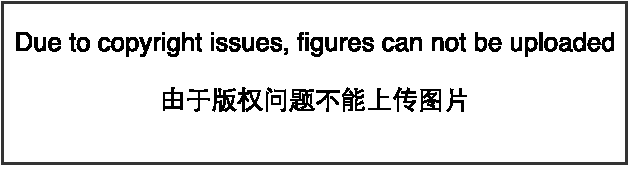
\includegraphics{figure.pdf}}
\else
\centerline{\includegraphics{Chapter9/figures/conv_layer}}
\fi
\caption{Tmp}
\label{fig:chap9_conv_layer}
\end{figure}

\gls{pooling}函数使用某一位置的相邻输出的总体统计特征来代替网络在该位置的输出。
例如,\firstgls{max_pooling} 函数\citep{zhou1988computation}给出相邻矩形区域内的最大值。
其他常用的\gls{pooling}函数包括相邻矩形区域内的平均值、$L^2$范数以及依靠据中心像素距离的加权平均函数。

% -- 330 --
 
不管采用什么样的\gls{pooling}函数,当输入做出微小平移时,\gls{pooling}能帮助我们的表示近似\firstgls{invariant}。
对于平移的不变性是说当我们把输入平移一微小的量,大多数通过\gls{pooling}函数的输出值并不会发生改变。
图\ref{fig:chap9_max_pool_invariance}用了一个例子来说明这是如何实现的。
\emph{局部平移不变性是一个很重要的性质,尤其是当我们关心某个特征是否出现而不关心它出现的具体位置时}。
例如,当判定一张图像中是否包含人脸时,我们并不需要知道眼睛的具体像素位置,我们只需要知道有一只眼睛在脸的左边,有一只在右边就行了。
但在一些其他领域,保存特征的具体位置却很重要。
例如当我们想要寻找一个由两条边相交而成的拐角时,我们就需要很好地保存边的位置来判定它们是否相交。
% fig 9.8
\begin{figure}[!htb]
\ifOpenSource
\centerline{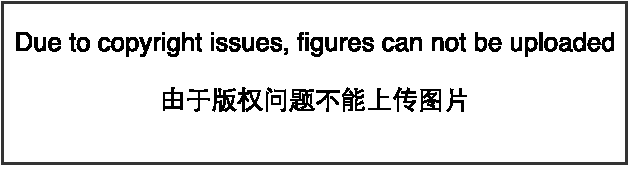
\includegraphics{figure.pdf}}
\else
\centerline{\includegraphics{Chapter9/figures/max_pool_invariance}}
\fi
\caption{Tmp}
\label{fig:chap9_max_pool_invariance}
\end{figure}

% -- 331 --
 
使用\gls{pooling}可以看作是增加了一个无限强的先验:卷积层学得的函数必须具有对于少量平移的不变性。
当这个假设成立时,\gls{pooling}可以极大地提高网络的统计效率。

\gls{pooling}对于空间区域具有平移不变性,但当我们对于分离参数的卷积输出进行\gls{pooling}时,特征能够学得应该对于哪种变换具有不变性(如图\ref{fig:chap9_learned_rotation}所示)。
% fig 9.9
\begin{figure}[!htb]
\ifOpenSource
\centerline{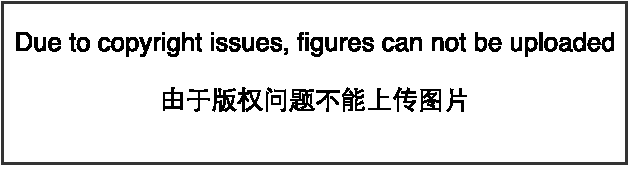
\includegraphics{figure.pdf}}
\else
\centerline{\includegraphics{Chapter9/figures/learned_rotation}}
\fi
\caption{Tmp}
\label{fig:chap9_learned_rotation}
\end{figure}

% -- 332 --
 
因为\gls{pooling}综合了全部邻居的反馈,这使得\gls{pooling}单元少于探测单元成为可能,我们可以通过综合\gls{pooling}区域的$k$个像素的统计特征而不是单个像素来实现。
图\ref{fig:chap9_pool_downsample}给出了一个例子。
这种方法提高了网络的计算效率,因为下一层少了约$k$ 倍的输入。
当下一层的参数数目是其输入大小的函数时(例如当下一层是全连接的依赖矩阵乘法的网络层时),这种对于输入规模的减小也可以提高统计效率并且减少对于参数的存储需求。
% fig 9.10
\begin{figure}[!htb]
\ifOpenSource
\centerline{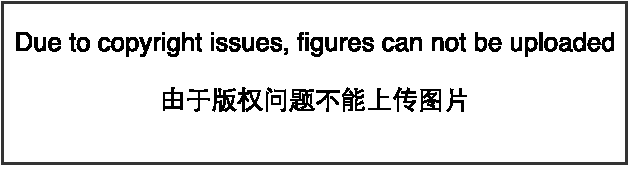
\includegraphics{figure.pdf}}
\else
\centerline{\includegraphics{Chapter9/figures/pool_downsample}}
\fi
\caption{Tmp}
\label{fig:chap9_pool_downsample}
\end{figure}

% -- 333 --
 
在很多任务中,\gls{pooling}对于处理不同大小的输入具有重要作用。
例如我们想对不同大小的图像进行分类时,分类层的输入必须是固定的大小,而这通常通过调整\gls{pooling}区域的偏置大小来实现,这样分类层总是能接收到相同数量的统计特征而不管最初的输入大小了。
例如,最终的\gls{pooling}层输出四个统计特征的集合,每个集合对应着图像的一个象限,而与图像的大小无关。

一些理论工作对于在不同情况下应当使用哪种\gls{pooling}函数给出了一些指导\citep{boureau-icml-10}。
动态地把特征\gls{pooling}在一起也是可行的,例如,通过针对特定属性的位置运行聚类算法\citep{boureau-iccv-11}。
这种方法对于每幅图像产生一个不同的\gls{pooling}区域集合。
另一种方法是先\emph{学习}一个单独的\gls{pooling}结构,再应用到全部的图像中\citep{jia2012beyond}。

\gls{pooling}可能会使得一些利用自顶向下信息的神经网络结构变得复杂,例如Boltzmann机和自动编码器。
这些问题将在第|||c|||部分中当我们遇到这些类型的网络时进一步讨论。
卷积Boltzmann机中的\gls{pooling}出现在\ref{sec:convolutional_boltzmann_machines}节。
一些可微网络中需要的在\gls{pooling}单元中进行的类逆运算将在\ref{sec:convolutional_generative_networks}节中讨论。

图\ref{fig:chap9_cnn_classifier}给出了一些使用卷积和\gls{pooling}操作的用于分类的\gls{CNN}的完整结构的例子。
% fig 9.11
\begin{figure}[!htb]
\ifOpenSource
\centerline{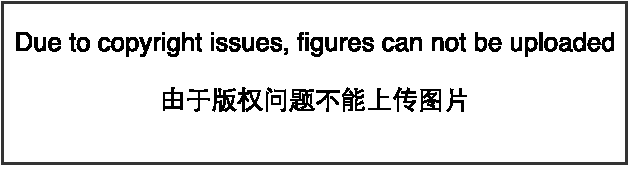
\includegraphics{figure.pdf}}
\else
\centerline{\includegraphics{Chapter9/figures/cnn_classifier}}
\fi
\caption{Tmp}
\label{fig:chap9_cnn_classifier}
\end{figure}

\section{卷积与\gls{pooling}作为一种无限强的先验}
\label{sec:convolution_and_pooling_as_an_infinitely_strong_prior}

回忆一下\ref{sec:capacity_overfitting_and_underfitting}节中\firstgls{prior_probability_distribution}的概念,这是一种在我们看到数据之前,将我们对于什么样的模型是合理的信念转化成的模型参数的概率分布。

% -- 334 --
 
先验被认为是强或者弱取决于先验中概率密度的集中程度。
弱先验具有较高的熵值,例如方差很大的Gaussian分布,这样的先验允许数据对于参数的改变具有或多或少的自由性。
强先验具有较低的熵值,例如方差很小的Gaussian分布,这样的先验在决定参数最终取值时起着更加积极的作用。

一个无限强的先验对一些参数的概率置零并且要求禁止对这些参数赋值,无论数据对于这些参数的值给出了多大的支持。

我们可以把\gls{CNN}想成一个相似的全连接网络,但对于它的权值有一个无限强的先验。
这个无限强的先验是说一个隐层单元的权值必须和它邻居的权值相等,但在空间中改变。
这个先验也要求除了在那些被指定到隐层单元中小的空间连续的接收域以外,其余的权值都为0。
总之,我们可以把卷积的使用当作是对网络中一层的参数引入了一个无限强的先验概率分布。
这个先验是说该层需要学得的函数具有局部连接和平移等价性。
类似的,使用\gls{pooling}也是一个无限强的先验:每一个单元都具有少量平移的不变性。

当然,把\gls{CNN}当作一个具有无限强先验的全连接网络来用会导致巨大的计算量浪费。
但把\gls{CNN}想成具有无限强先验的全连接网络可以帮助我们更好地理解\gls{CNN}是如何工作的。

其中一个关键点是卷积和\gls{pooling}可能导致欠拟合。
与任何先验类似,卷积和\gls{pooling}只有当先验的假设合理且正确时才有用。
如果一项任务依赖于保存精确的空间信息,那么在所有的特征上使用\gls{pooling}都会增大训练误差。
一些\gls{CNN}\citep{Szegedy-et-al-arxiv2014}为了同时获得具有较高不变性的特征以及当平移不变性不合理时不会导致欠拟合的特征,被设计成在一些通道上使用\gls{pooling}而在另一些通道上不使用。
当一项任务涉及到要对输入中相隔较远的信息进行合并时,那么卷积所需要的先验可能就不正确了。

另一个关键点是我们在比较卷积模型的统计学习表现时,只能以基准中的卷积模型作为比较的对象。
其他不使用卷积的模型即使我们把图像中的所有像素点都置换后依然有可能进行学习。
对于许多图像数据集,具有\firstgls{permutation_invariant}并且必须通过学习发现拓扑结构的模型也有一些基准,还有一些模型他们的设计者将空间关系的知识通过硬编码给了它们。

% -- 336 --

\section{基本卷积函数的变体}
\label{sec:variants_of_the_basic_convolution_function}

当在神经网络的上下文中讨论卷积时,我们通常不会像数学文献中那样特指标准的离散卷积运算。
实际应用中的函数略微有些不同。
这里我们详细讨论一下这些差异,并且对神经网络中用到的函数的一些重要性质进行重点说明。

首先,当我们提到神经网络中的卷积时,我们通常是指一次特定的运算,而这种运算包含了多个卷积应用的并行处理。
这是因为带有单个核的卷积只能提取一种类型的特征,尽管它作用在多个空间位置上。
我们通常希望神经网络的一层能够在多个位置提取多种类型的特征。

另外,输入通常也不仅仅是实值的方格,而是由一系列向量值的观测数据构成的方格。
例如,一幅彩色图像在每一个像素点都会有红绿蓝三种颜色的亮度。
在多层的\gls{CNN}中,第二层的输入是第一层的输出,通常包含多个卷积作用后的输出。
当用于图像时,我们通常把卷积的输入输出都看作是3维的张量,其中一个索引用于标明不同的通道(红绿蓝),另外两个索引标明在这个通道上的空间坐标。
软件实现通常使用批处理模式,所以它们会使用4维的张量,第四维索引用于标明批处理中不同的实例,但我们为简明起见这里忽略批处理索引。

因为\gls{CNN}通常使用多通道的卷积,它们基于的线性运算并不保证一定是可交换的,即使使用了核翻转也是如此。
这些多通道的运算只有当其中的每个运算的输出和输入具有相同的通道数时才是可交换的。

假定我们有一个4维的核张量$\TSK$,它的每一个元素是$\TEK_{i,j,k,l}$,表示输出的在通道$i$中的一个单元和输入的在通道$j$中的一个单元的连接强度,并且在输出单元和输入单元之间有一个$k$ 行$l$ 列的偏置。
假定我们的输入是观测数据$\TSV$,它的每一个元素是$\TEV_{i,j,k}$,表示在通道$i$中第$i$行第$j$列的值。
假定我们的输出$\TSZ$和输入$\TSV$具有相同的形式。
如果输出$\TSZ$是通过对$\TSK$和$\TSV$进行卷积而不涉及翻转$\TSK$得到的,那么
\begin{equation}
\TEZ_{i,j,k} = \sum_{l,m,n} \TEV_{l, j+m-1, k+n-1} \TEK_{i,l,m,n}
\end{equation}
这里对所有的$l$,$m$和$n$进行求和也是对所有有效的张量索引的值进行求和。
在线性代数中,向量中的索引通常从1开始,这就是上述公式中$-1$的由来。
但是像C或Python这类编程语言索引通常从0开始,这使得上述公式可以更加简洁。

% -- 337 --
 
我们有时会希望跳过核中的一些位置来降低计算的开销(相应的代价是提取特征没有先前那么好了)。
我们可以把这一过程看作是对卷积函数输出的下采样。
如果我们只想对输出的每个方向上的$s$个像素进行采样,那么我们可以定义一个下采样卷积函数$c$使得
\begin{equation}
\TEZ_{i,j,k} = c(\TSK, \TSV, s)_{i,j,k} = \sum_{l,m,n} [\TEV_{l,(j-1)\times s+m, (k-1)\times s +n,}
 \TEK_{i,l,m,n}].
 \label{eq: 9.8}
\end{equation}
我们把$s$称为下采样卷积的\firstgls{stride}。
当然也可以对每个方向定义不同的步幅。
图\ref{fig:chap9_stride_conv}演示了一个实例。
% fig 9.12
\begin{figure}[!htb]
\ifOpenSource
\centerline{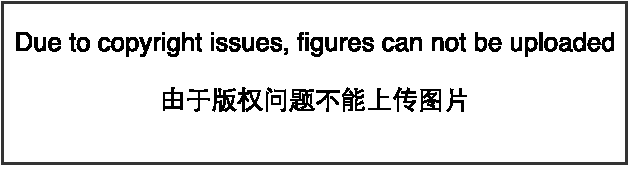
\includegraphics{figure.pdf}}
\else
\centerline{\includegraphics{Chapter9/figures/stride_conv}}
\fi
\caption{Tmp}
\label{fig:chap9_stride_conv}
\end{figure}

在任何\gls{CNN}的应用中都有一个重要性质,那就是能够隐含地对输入$\TSV$用零进行填充使得它加宽。
如果没有这个性质,表示的宽度在每一层就会缩减,缩减的幅度是比核少一个像素这么多。
对输入进行零填充允许我们对核的宽度和输出的大小进行独立的控制。
如果没有零填充,我们就被迫面临网络空间长度的快速缩减和选择一个小型的核的两难的局面——这两种情境都会极大得限制网络的表示能力。
图\ref{fig:chap9_zero_pad_shrink}给出了一个例子。
% fig 9.13
\begin{figure}[!htb]
\ifOpenSource
\centerline{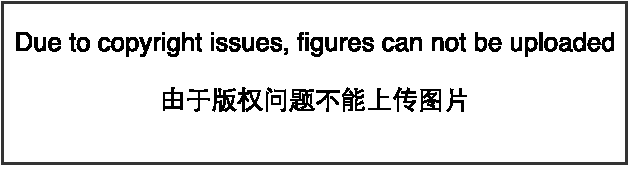
\includegraphics{figure.pdf}}
\else
\centerline{\includegraphics{Chapter9/figures/zero_pad_shrink}}
\fi
\caption{Tmp}
\label{fig:chap9_zero_pad_shrink}
\end{figure}

有三种零填充设定的情况值得注意。
第一种是无论怎样都不使用零填充的极端情况,并且卷积核只允许访问那些图像中能够完全包含整个核的位置。
在MATLAB中,这称为\firstgls{valid}卷积。
在这种情况下,输出的所有像素都是输入中相同数量像素的函数,这使得输出像素的表现更加规范。
然而,输出的大小在每一层都会缩减。
如果输入的图像宽度是$m$,核的宽度是$k$,那么输出的宽度就会变成$m-k+1$。
如果卷积核非常大的话缩减率会非常显著。
因为缩减数大于0,这限制了网络中的卷积层的层数。
当层数增加时,网络的空间维度最终会缩减到$1\times 1$,这种情况下其他的层就不可能进行有意义的卷积了。
第二种特殊的情况是只进行足够的零填充来保持输出和输入具有相同的大小。
在MATLAB中,这称为\firstgls{same}卷积。
在这种情况下,网络能够包含足够多的卷积层,只要硬件可以支持,这是因为卷积运算并没有改变相关的结构。
然而,输入像素中靠近边界的部分相比于中间部分对于输出像素的影响更小。
这可能会导致边界像素存在一定程度的欠表示。
这使得第三种极端情况产生了,在MATLAB中称为\firstgls{full}卷积。
它是对每个方向上被访问了$k$次的像素进行足够的零填充,最终输出的图像的宽度为$m+k-1$。
在这种情况下,输出像素中靠近边界的部分相比于中间部分是更少像素的函数。
这将导致学得一个在卷积特征图的所有位置都表现不错的单核更为困难。
通常零填充的最优数量(对于测试集的分类正确率)处于``有效卷积''和``相同卷积''之间的某个位置。

% -- 338 --
 
% -- 339 --

在一些情况下,我们并不一定真正想用卷积,而只是用一些局部连接的网络层\citep{LeCun86,LeCun89a}。
在这种情况下,我们的多重感知机对应的邻接矩阵是相同的,但每一个连接都有它自己的权重,用一个6维的张量$\TSW$来表示。
$\TSW$的索引分别是:输出的通道$i$,输出的行$j$和列$k$,输入的通道$l$,输入的行偏置$m$和列偏置$n$。
局部连接层的线性部分可以表示为
\begin{equation}
\TEZ_{i,j,k} = \sum_{l,m,n} [\TEV_{l, j+m-1, k+n-1} w_{i, j, k, l, m, n}].
\end{equation}
这有时也被称为\firstgls{unshared_convolution},因为它和带有一个小核的离散卷积运算很像,但并不横跨位置来共享参数。
图\ref{fig:chap9_local}比较了局部连接、卷积和全连接的区别。
% fig 9.14
\begin{figure}[!htb]
\ifOpenSource
\centerline{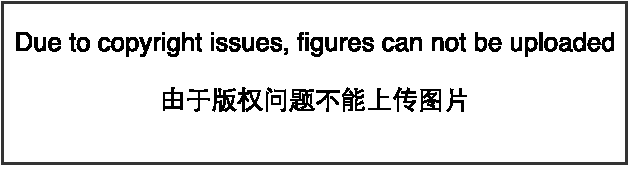
\includegraphics{figure.pdf}}
\else
\centerline{\includegraphics{Chapter9/figures/local}}
\fi
\caption{Tmp}
\label{fig:chap9_local}
\end{figure}
 
% -- 340 --
 
当我们知道每一个特征都是一小部分空间的函数而不是整个空间的特征时,局部连接层是很有用的。
例如,如果我们想要辨别一张图片是否是人脸图像时,我们只需要去寻找嘴是否在图像的下部的居中部分即可。

在连接被更进一步限制时,使用一些新版本的卷积或者局部连接层是有用的,例如,当每一个输出的通道$i$被限制成仅仅是输入的一部分通道$l$的函数时。
处理这种情况的一种通用方法是使输出的前$m$个通道仅仅连接到输入的前$n$个通道,输出的接下来的$m$个通道仅仅连接到输入的接下来的$n$个通道,以此类推。
如图\ref{{fig:chap9_conv_groups}}所示。
对少量通道的连接进行建模允许网络使用更少的参数来降低存储的消耗以及提高统计效率,并且减少了前向和后向传播所需要的计算量。
这些目标的实现并没有减少隐藏单元的数目。
% fig 9.15
\begin{figure}[!htb]
\ifOpenSource
\centerline{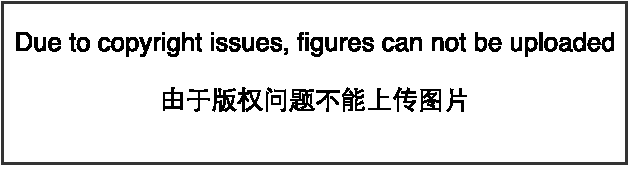
\includegraphics{figure.pdf}}
\else
\centerline{\includegraphics{Chapter9/figures/conv_groups}}
\fi
\caption{Tmp}
\label{fig:chap9_conv_groups}
\end{figure}

\firstgls{tiled_convolution}\citep{Gregor+LeCun-2010,Le2010}对卷积层和局部连接层进行了折衷。
这里并不是对\emph{每一个}空间位置的权重进行学习,我们学习一些核使得当我们在空间移动时它们可以循环利用。
这意味着在最近邻的位置拥有不同的滤波器,就像局部连接层一样,但是对于这些参数的存储需求仅仅会随着核的集合的大小成常数倍增长,而不是整个输出的特征图的大小。
图\ref{fig:chap9_tiled}对局部连接层、尾卷积和标准卷积进行了比较。
% fig 9.16
\begin{figure}[!htb]
\ifOpenSource
\centerline{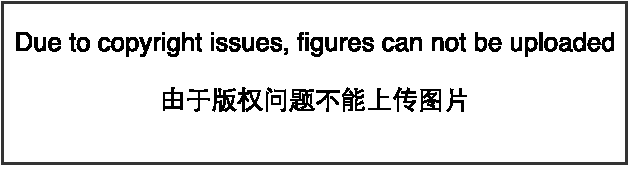
\includegraphics{figure.pdf}}
\else
\centerline{\includegraphics{Chapter9/figures/tiled}}
\fi
\caption{Tmp}
\label{fig:chap9_tiled}
\end{figure}
 
% -- 341 --
 
为了代数化地定义尾卷积,令$k$是一个6维的张量,其中的两维对应着输出图中的不同位置。
我们这里并不是使用离散的索引来表示输出图中的每一个位置,输出的位置在每个方向上在$t$个不同的核的栈组成的集合中进行循环。
如果$t$等于输出的宽度,这就和局部连接层等价了。
\begin{equation}
\TEZ_{i, j, k} = \sum_{l, m, n} \TEV_{l, j+m-1, k+n-1} \TEK_{i, l, m, n, j\% t +1, k\% t+1},
\end{equation}
这里$\%$是模运算,并且$t\% t =0, (t+1)\% t = 1$等等。
在每一维上使用其他的索引方法可以很直观的对这个方程进行扩展。
 
% -- 342 --
  
% -- 343 --
 
局部连接层和尾卷积层都和最大\gls{pooling}有一些有趣的关联:这些层的探测单元都是由不同的过滤器驱动的。
如果这些过滤器能够学会对相同隐藏特征的不同变换形式进行探测,那么最大\gls{pooling}的单元对于学得的变换就具有不变性(如图\ref{fig:chap9_learned_rotation}所示)。
卷积层对于平移具有内置的不变性。
 
% -- 344 --
 
使用\gls{CNN}时,采用除卷积以外的其他一些运算通常也是必须的。
为了实现学习,必须在给定输出的梯度时能够计算核的梯度。
在一些情况下,这种运算可以通过卷积来实现,但在很多我们感兴趣的情况下,包括步幅大于1的情况,并不具有这样的性质。

回忆一下卷积是一种线性运算,所以可以表示成矩阵乘法的形式(如果我们首先把输入张量变形为一个单纯的向量)。
涉及到的矩阵是卷积核的函数。
这个矩阵是稀疏的并且核的每个元素都复制给矩阵的很多个元素。
这种观点能够帮助我们导出\gls{CNN}需要的很多其他运算。

通过卷积定义的矩阵转置的乘法就是这样一种运算。
这种运算用于在卷积层中后向传播误差的导数,所以可以用来训练多于一个隐含层的\gls{CNN}。
如果我们想要从隐藏层单元来重构可视化单元时,同样的运算也是需要的\citep{Simard92-short}。
重构可视化单元是本书第|||c|||部分的模型广泛用到的一种运算,这些模型包括自动编码器、RBM和稀疏编码等等。
构建这些模型的卷积化的版本都要用到转置化卷积。
就像核梯度的运算,这种输入梯度运算在某些情况下可以用卷积来实现,但在一般情况下需要用到第三种运算来实现。
必须非常小心地来使这种转置运算和前向传播过程相协调。
转置运算返回的输出的大小取决于三个方面:零填充的策略、前向传播运算的步幅和前向传播的输出映射的大小。
在一些情况下,不同大小的输入通过前向传播过程能够得到相同大小的输出映射,所以必须明确地告知转置运算原始输入的大小。

这三个运算——卷积、从输出到权值的后向传播和从输出到输入的后向传播——足以计算任何深度的前馈\gls{convolutional_network}训练所需的梯度,也可以计算带有基于转置化卷积的重构函数的\gls{convolutional_network}训练所需的梯度。
对于完全一般的多维、多样例情况下的公式的完整推导可以参见\cite{Goodfellow-TR2010}。 
为了直观说明这些公式是如何起作用的,我们这里给出一个二维单样例的版本。
 
% -- 345 --
 
假设我们想要训练这样一个\gls{CNN},它包含带有步幅的卷积并且步幅为$s$,该卷积的核$\TSK$作用于多通道的图像$\TSV$,表示为$c(\TSK, \TSV, s)$就像公式\ref{eq: 9.8}中一样。
假设我们想要最小化某个损失函数$J(\TSV, \TSK)$。
在前向传播过程中,我们需要用$c$本身来输出$\TSZ$,然后$\TSZ$传递到网络的其余部分并且被用来计算损失函数$J$。
在后向传播过程中,我们会收到一个张量$\TSG$表示为$\TEG_{i, j, k} = \frac{\partial}{\partial \TEZ_{i, j, k}} J(\TSV, \TSK)$。

为了训练网络,我们需要对核中的权值分别求导。
为了实现这个目的,我们可以使用一个函数
\begin{equation}
g(\TSG, \TSV, s)_{i, j, k, l} = \frac{\partial}{\partial \TEK_{i, j, k, l}} J(\TSV, \TSK) = \sum_{m, n} \TEG_{i, m, n} \TEV_{j, (m-1)\times s+k, (n-1)\times s+l}.
\end{equation}

如果这一层不是网络的底层,我们需要对$\TSV$求梯度来使得误差后向传播。
我们可以使用如下的函数
\begin{eqnarray}
h(\TSK, \TSG, s)_{i, j, k} &=& \frac{\partial }{\partial \TEV_{i, j, k}} J(\TSV, \TSK)\\
&=& \sum_{\substack{l, m\\
                  \text{s.t.}\\
                  (l-1)\times s+m = j}} \sum_{\substack{n, p\\
                                                            \text{s.t.}\\
                                                            (n-1)\times s +p = k}}
            \sum_q \TEK_{q,i,m,p} \TEG_{q, l, n}.
\end{eqnarray}

第\ref{chap:autoencoders}章描述的自动编码器网络,是一些训练成把输入拷贝到输出的前馈网络。
一个简单的例子是PCA算法,将输入$\bm{x}$拷贝到一个近似的重构值$\bm{r}$,通过函数$\bm{W}^\top \bm{Wx}$来实现。
使用带有矩阵转置的乘法,就像PCA算法这种,在一般的自动编码器中是很常见的。
为了使这些模型卷积化,我们可以用函数$h$来实现卷积运算的转置。
假定我们有和$\TSZ$相同格式的隐藏单元$\TSH$,并且我们定义一种重构运算
\begin{equation}
\TSR = h(\TSK, \TSH, s).
\end{equation}

为了训练自动编码器,我们会收到关于$\TSR$的梯度表示为一个张量$\TSE$。
为了训练解码器,我们需要获得对于$\TSK$的梯度,通过$g(\TSH, \TSE, s)$来得到。
为了训练编码器,我们需要获得对于$\TSH$的梯度,通过$c(\TSK, \TSE, s)$来得到。
也可能通过用$c$和$h$对$g$求微分得到,但这些运算对于任何标准神经网络上的后向传播算法来说都是不需要的。
 
% -- 346 --
 
一般来说,在卷积层从输入到输出的变换中我们不仅仅只用线性运算。
我们一般也会在进行非线性运算前对每个输出加入一些偏置项。
这样就产生了如何在偏置项中共享参数的问题。
对于局部连接层,对于每个单元都给定它特有的偏置是很自然的,对于尾卷积,用与核一样的方式来共享参数也是很自然的。
对于卷积层来说,典型的做法是在输出的每一个通道上都设置一个偏置,这个偏置在每个卷积映射中的所有位置进行共享。
然而,如果输入是已知的固定大小,也可以在输出映射的每个位置学习一个单独的偏置。
分离这些偏置可能会稍稍降低模型的统计效率,但同时也允许模型来校正图像中不同位置的统计差异。
例如,当使用零填充时,图像边缘的探测单元接收到较少的输入,因此需要较大的偏置。

\section{结构化输出}
\label{sec:structured_outputs}

\gls{CNN}可以用于输出高维的结构化对象,而不仅仅是预测分类任务的类标签或回归任务的实际值。
通常这个对象只是一个张量,由标准卷积层产生。
例如,模型可以产生张量$\TSS$,其中$\TES_{i,j,k}$是网络的输入像素$(j, k)$属于类$i$的概率。
这允许模型标记图像中的每个像素,并绘制遵循单个对象轮廓的精确掩模。

经常出现的一个问题是输出平面可能比输入平面要小,如图\ref{fig:chap9_zero_pad_shrink}所示。
在通常用于图像中单个对象分类的各种结构中,网络空间维数的最大减少来源于使用具有大步幅的\gls{pooling}层。
为了产生与输入大小相似的输出映射,可以避免完全的\gls{pooling}\citep{jain2007supervised}。
另一种策略是简单地产生低分辨率的标签网格\citep{Pinheiro+Collobert-ICML2014,Pinheiro+Collobert-CVPR2015}。
最后,原则上,可以使用具有单位步长的\gls{pooling}操作。

用于图像中逐个像素标记的一种策略是先产生图像标签的原始猜测,然后使用相邻像素之间的交互来修正该原始猜测。
重复这个修正步骤几次对应于在每一步使用相同的卷积,在深层网络的最后几层之间共享权重\citep{jain2007supervised}。
这使得在层之间共享参数的连续\gls{convolutional_network}执行的一系列运算,形成了一种特殊的循环神经网络\citep{Pinheiro+Collobert-ICML2014,Pinheiro+Collobert-CVPR2015}。
图\ref{fig:chap9_iterative}给出了这样一个循环\gls{convolutional_network}的结构。
% fig 9.17
\begin{figure}[!htb]
\ifOpenSource
\centerline{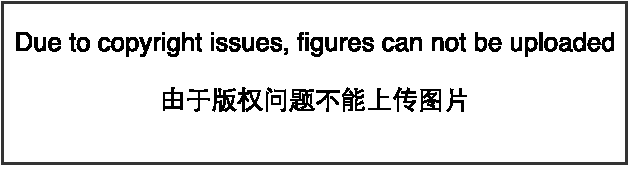
\includegraphics{figure.pdf}}
\else
\centerline{\includegraphics{Chapter9/figures/iterative}}
\fi
\caption{Tmp}
\label{fig:chap9_iterative}
\end{figure}

% -- 347 --
 
一旦对每个像素都进行了预测,可以使用各种方法来进一步处理这些预测,以便获得图像区域上的分割\citep{Briggman-et-al-NIPS2009,Turaga2010,Farabet-et-al-2013}。
一般的想法是假设大组连续的像素倾向于对应着相同的标签。
图模型可以描述相邻像素之间的概率关系。
或者,\gls{convolutional_network}可以被训练来最大化地近似图模型训练的目标\citep{Ning-et-al-2005,Thompson-et-al-NIPS2014}。

\section{数据类型}
\label{sec:data_types}

\gls{convolutional_network}使用的数据通常包含多个通道,每个通道是在时间或空间中的某一点观测到的一个不同的量。
参见表|||c|||来了解具有不同维数和通道数的数据类型的例子。
 
% -- 348 --
  
% -- 349 --
 
\gls{convolutional_network}用于视频的例子,可以参见\cite{Chen-Ting-2010}。

到目前为止,我们仅讨论了训练和测试数据中的每个样例都有相同的空间维度的情况。
\gls{convolutional_network}的一个优点是它们还可以处理具有变化的空间范围的输入。
这些类型的输入不能用传统的基于矩阵乘法的神经网络来表示。
这提供了使用\gls{convolutional_network}的令人信服的理由,即使当计算成本和过拟合不是主要问题时。

例如,考虑一组图像的集合,其中每个图像具有不同的高度和宽度。
目前还不清楚如何用固定大小的权重矩阵对这样的输入进行建模。
卷积就可以很直观的应用;核依据输入的大小简单地被使用不同次,并且卷积运算的输出也相应地放缩。
卷积可以被视为矩阵乘法;相同的卷积核为每种大小的输入包含一个不同大小的双重块循环矩阵。
有时,网络的输出允许和输入一样具有可变的大小,例如如果我们想要为输入的每个像素分配一个类标签。
在这种情况下,不需要进一步的设计工作。
在其他情况下,网络必须产生一些固定大小的输出,例如,如果我们想要为整个图像指定单个类标签。
在这种情况下,我们必须进行一些额外的设计步骤,例如插入一个\gls{pooling}层,\gls{pooling}区域的大小要与输入的大小成比例,以便保持固定数量的\gls{pooling}输出。
这种策略的一些例子可以参见图\ref{fig:chap9_cnn_classifier}。

注意,使用卷积处理可变尺寸的输入仅对具有尺寸可变的输入才有意义,因为它们包含对相同种类的事物的不同量的观察——时间上不同长度的记录,空间上不同宽度的观察等。
如果输入具有可变尺寸,卷积是没有意义的,因为它可以选择性地包括不同种类的观察。
例如,如果我们正在处理大学申请,并且我们的特征包括成绩和标准化测试分数,但不是每个申请人都进行了标准化测试,则使用相同的权重来对成绩特征和测试分数特征进行卷积是没有意义的。

\section{高效的卷积算法}
\label{sec:efficient_convolution_algorithms}

现代\gls{convolutional_network}的应用通常涉及包含超过百万个单元的网络。
强大的实现要利用并行计算资源,很关键的,如\ref{sec:large_scale_deep_learning}节中所描述。
然而,在很多情况下,也可以通过选择适当的卷积算法来加速卷积。
 
% -- 350 --
 
卷积等效于使用Fourier变换将输入与核都转换到频域,执行两个信号的逐点相乘,并使用Fourier逆变换转换回时域。
对于某些问题大小,这可能比离散型卷积的朴素实现更快。

当一个$d$维的核可以表示成$d$个向量(每维一个向量)的外积时,该核称为\firstgls{separable}。
当核可分离时,朴素的卷积是低效的。
它等价于组合$d$个一维卷积,每个卷积使用这些向量中的一个。
组合方法显著快于使用它们的外积来执行一个$d$维的卷积。
并且核也需要更少的参数表示为向量。
如果核在每一维都是$w$个元素宽,那么朴素的多维卷积需要$O(w^d)$的运行时间和参数存储空间,而可分离卷积只需要$O(w\times d)$的运行时间和参数存储空间。
当然,并不是每个卷积都可以表示成这种形式。

设计更快的执行卷积或近似卷积,而不损害模型准确性的方法,是一个活跃的研究领域。 
甚至仅提高前向传播效率的技术也是有用的,因为在商业环境中,通常部署网络比训练网络还要耗资源。

\section{随机或无监督的特征}
\label{sec:random_or_unsupervised_features}

通常,\gls{convolutional_network}训练中最昂贵的部分是学习特征。 
输出层通常相对便宜,因为在通过若干层\gls{pooling}之后作为该层输入的特征的数量较少。
当使用梯度下降执行有监督训练时,每个梯度步骤需要完整的运行前向传播和后向传播通过整个网络。
减少\gls{convolutional_network}训练成本的一种方式是使用那些不是通过有监督方式训练的特征。

有三种基本策略不通过有监督训练而得到卷积核。
其中一个是简单地随机初始化它们。
另一个是手动设计它们,例如设置每个核在一个特定的方向或尺度来检测边缘。
最后,可以使用无监督的标准来学习核。
例如,\cite{Coates2011}将$k$均值聚类算法应用于小图像块,然后使用每个学得的中心作为卷积核。
第|||c|||部分描述了更多的无监督学习方法。
使用无监督标准学习特征,允许它们的确定与位于网络结构顶层的分类层相分离。
然后只需提取一次全部训练集的特征,构造用于最后一层的新训练集。
假设最后一层类似logistic回归或者SVM,那么学习最后一层通常是凸优化问题。
 
% -- 351 --
 
随机过滤器经常在\gls{convolutional_network}中表现得出乎意料得好\cite{Jarrett-ICCV2009-small,Saxe-ICML2011,pinto2011scaling,cox2011beyond}。
\cite{Saxe-ICML2011}说明,由卷积和随后的\gls{pooling}组成的层,当赋予随机权值时,自然地变得具有频率选择和平移不变性。
他们认为这提供了一种廉价的方法来选择\gls{convolutional_network}的结构:首先通过仅训练最后一层来评估几个\gls{convolutional_network}结构的性能,然后选择最好的结构并使用更昂贵的方法来训练整个网络。

一个中间方法是学习特征,但是使用一些特殊的方法,这些方法不需要在每个梯度步骤中都进行完整的前向和后向传播。
与多层感知机一样,我们使用贪心逐层式预训练,独立地训练第一层,然后从第一层提取所有特征一次,然后用那些特征隔离训练第二层,以此类推。
第\ref{chap:optimization_for_training_deep_models}章描述了如何实现有监督的贪心逐层预训练,第|||c|||部分将此扩展到了无监督的范畴。
卷积模型的贪心逐层预训练的经典模型是卷积深度信念网络\citep{HonglakL2009}。
\gls{convolutional_network}为我们提供了相对于多层感知机更进一步采用预训练策略的机会。
不是一次训练整个卷积层,我们可以训练一小块模型,就像\cite{Coates2011}使用$k$均值做的那样。
然后,我们可以用来自这个小块模型的参数来定义卷积层的核。
这意味着使用无监督学习来训练\gls{convolutional_network}\textbf{并且在训练的过程中完全不使用卷积}是可能的。
使用这种方法,我们可以训练非常大的模型,并且只在推理期间产生高计算成本\citep{ranzato-cvpr-07-small,Jarrett-ICCV2009-small,koray-nips-10-small,icml2013_coates13}。
这种方法从2007年到2013年流行,当时标记的数据集很小,并且计算能力更有限。
如今,大多数\gls{convolutional_network}以纯粹有监督的方式训练,在每次训练迭代中使用通过整个网络的完整的前向和反向传播。
 
% -- 352 --
 
与其他无监督预训练的方法一样,使用这种方法的一些好处仍然难以说清。
无监督预训练可以提供一些相对于有监督训练的正则化,或者它可以简单地允许我们训练更大的结构,因为它的学习规则减少了计算成本。

\section{\gls{CNN}的神经科学基础}
\label{sec:the_neuroscientific_basis_for_convolutional_networks}

\gls{convolutional_network}也许是生物学启发人工智能的最为成功的故事。
虽然\gls{convolutional_network}已经被许多其他领域指导,但是神经网络的一些关键设计原则来自神经科学。

\gls{convolutional_network}的历史始于神经科学实验,远早于相关计算模型的发展。
神经生理学家David Hubel和Torsten Wiesel合作多年,为了确定关于哺乳动物视觉系统如何工作的许多最基本的事实\citep{Hubel+Wiesel-1959,Hubel62,Hubel+Wiesel-1968}。
他们的成就最终获得了诺贝尔奖。
他们的发现对当代深度学习模型有最大影响的是基于记录猫的单个神经元的活动。
他们观察了猫的脑内神经元如何响应投影在猫前面屏幕上精确位置的图像。
他们的伟大发现是,处于视觉系统较为前面的神经元对非常特定的光模式(例如精确定向的条纹)反应最强烈,但对其他模式几乎完全没有反应。

他们的工作有助于表征大脑功能的许多方面,这些方面超出了本书的范围。
从深度学习的角度来看,我们可以专注于简化的,卡通形式的大脑功能视图。

在这个简化的视图中,我们关注被称为V1的大脑的一部分,也称为\firstgls{primary_visual_cortex}。
V1是大脑对视觉输入开始执行显著高级处理的第一个区域。
在该卡通视图中,图像是由光到达眼睛并刺激视网膜(眼睛后部的光敏组织)形成的。
视网膜中的神经元对图像执行一些简单的预处理,但是基本不改变它被表示的方式。
然后图像通过视神经和称为外侧膝状核的脑部区域。 
这些解剖区域的主要作用是仅仅将信号从眼睛传递到位于头后部的V1。
 
% -- 353 --
 
\gls{convolutional_network}层被设计为描述V1的三个性质:
\begin{enumerate}
  \item V1布置在空间图中。
  它实际上具有二维结构来反映视网膜中的图像结构。
  例如,到达视网膜下半部的光仅影响V1相应的一半。 
  \gls{convolutional_network}通过用二维映射定义特征的方式来描述该特性。

  \item V1包含许多\firstgls{simple_cells}。
  简单细胞的活动在某种程度上可以概括为在一个小的空间位置接受域内的图像的线性函数。
  \gls{convolutional_network}的检测器单元被设计为模拟简单细胞的这些性质。

  \item V1还包括许多\firstgls{complex_cells}。
  这些细胞响应类似于由简单细胞检测的那些特征,但是复杂细胞对于特征的位置微小偏移具有不变性。 
  这启发了\gls{convolutional_network}的\gls{pooling}单元。
  复杂细胞对于照明中的一些变化也是不变的,不能简单地通过在空间位置上\gls{pooling}来刻画。 
  这些不变性激发了\gls{convolutional_network}中的一些跨通道\gls{pooling}策略,例如maxout单元\citep{Goodfellow-et-al-ICML2013}。
\end{enumerate}

虽然我们最了解V1,但是一般认为相同的基本原理也适用于视觉系统的其他区域。
在我们视觉系统的卡通试图中,当我们逐渐深入大脑时,遵循\gls{pooling}的基本探测策略被反复执行。
当我们穿过大脑的多个解剖层时,我们最终找到了响应一些特定概念的细胞,并且这些细胞对输入的很多种变换都具有不变性。
这些细胞被昵称为``祖母细胞''——这个想法是一个人可能有一个神经元,当看到他祖母的照片时该神经元被激活,无论祖母是出现在照片的左边或右边,无论照片是她的脸部的特写镜头还是她的全身照,也无论她处在光亮还是黑暗中,等等。

这些祖母细胞已经被证明确实存在于人脑中,在一个被称为\emph{内侧颞叶}的区域\citep{quiroga2005invariant}。
研究人员测试了单个神经元是否会响应名人的照片。
他们发现了后来被称为``Halle Berry神经元''的神经元:由Halle Berry的概念激活的单个神经元。
当一个人看到Halle Berry的照片,Halle Berry的图画,甚至包含单词``Halle Berry''的文本时,这个神经元会触发。
当然,这与Halle Berry自己无关;其他神经元响应Bill Clinton,Jennifer Aniston等的出现。
 
% -- 354 --
 
这些内侧颞叶神经元比现代\gls{convolutional_network}更通用,它们在读取名称时不会自动推广到识别人或对象。
与\gls{convolutional_network}的最后一层特征上最接近的类比是称为颞下皮质(IT)的脑区。
当查看一个物体时,信息从视网膜经LGN流到V1,然后到V2,V4,然后是IT。
这发生在瞥见物体的前100ms内。
如果允许一个人继续观察物体更多的时间,那么信息将开始向后流动,因为大脑使用自上而下的反馈来更新较低级脑区中的激活。
然而,如果我们打断人的注视,并且只观察前100ms内的大多数前向激活导致的放电率,那么IT被证明与\gls{convolutional_network}非常相似。
\gls{convolutional_network}可以预测IT放电率,并且在执行物体识别任务时与人类(时间有限的情况)非常类似\citep{dicarlo-tutorial-2013}。

话虽如此,\gls{convolutional_network}和哺乳动物的视觉系统之间还是有许多区别。
这些区别有一些是计算神经科学家所熟知的,但超出了本书的范围。
还有一些区别尚未知晓,因为关于哺乳动物视觉系统如何工作的许多基本问题仍未得到回答。
简要列表如下:
\begin{itemize}
  \item 人眼大部分是非常低的分辨率,除了一个被称为\firstgls{fovea}的小块。
  中央凹仅观察保持在手臂长度的拇指大小的区域。
  虽然我们觉得我们可以看到高分辨率的整个场景,但这是由我们的大脑的潜意识部分创建的错觉,因为它缝合了我们瞥见的若干个小区域。
  大多数\gls{convolutional_network}实际上接收大的全分辨率的照片作为输入。
  人类大脑控制几次眼动,称为\firstgls{saccade},以瞥见场景中最显眼的或任务相关的部分。
  将类似的关注机制融入深度学习模型是一个活跃的研究方向。
  在深度学习的背景下,关注机制对于自然语言处理是最成功的,参见\ref{sec:using_an_attention_mechanism_and_aligning_pieces_of_data}节。
  已经研发了几种具有视觉机制的视觉模型,但到目前为止还没有成为主导方法\citep{Larochelle2010,Denil2012}。
  
  \item 人类视觉系统集成了许多其他感觉,例如听觉,以及像我们的心情和想法一样的因素。
  \gls{convolutional_network}迄今为止纯粹是视觉的。
  
  \item 人类视觉系统不仅仅用于识别对象。
  它能够理解整个场景,包括许多物体和物体之间的关系,以及处理我们的身体与世界交互所需的丰富的三维几何信息。
  \gls{convolutional_network}已经应用于这些问题中的一些,但是这些应用还处于起步阶段。
  
  \item 即使像V1这样简单的大脑区域也受到来自较高级别的反馈的严重影响。
  反馈已经在神经网络模型中被广泛地探索,但还没有被证明提供了引人注目的改进。
  
  \item 虽然前馈IT放电频率刻画了与\gls{convolutional_network}特征很多相同的信息,但是仍不清楚中间计算的相似程度。
  大脑可能使用非常不同的激活和\gls{pooling}函数。
  单个神经元的激活可能不能用单个线性过滤器的响应来很好地表征。
  最近的V1模型涉及对每个神经元的多个二次过滤器\citep{rust:2005}。
  事实上,我们的``简单细胞''和``复杂细胞''的卡通图片可能并没有区别;简单细胞和复杂细胞可能是相同种类的细胞,但是它们的``参数''使得它们能够实现从我们所说的``简单''到``复杂''的连续的行为。
\end{itemize}
 
% -- 355 --
 
还值得一提的是,神经科学很少告诉我们该如何\emph{训练}\gls{convolutional_network}。
具有跨多个空间位置的\gls{parameter_sharing}的模型结构,可以追溯到早期关于视觉的联结主义模型\citep{Marr76},但是这些模型没有使用现代的反向传播算法和梯度下降。
例如,\citep{Fukushima80}结合了现代\gls{convolutional_network}的大多数模型结构设计元素,但依赖于层次化的无监督聚类算法。

\cite{Lang+Hinton88}引入反向传播来训练\firstall{TDNNs}。
使用当代术语来说,TDNNs 是用于时间序列的一维\gls{convolutional_network}。
用于这些模型的反向传播不受任何神经科学观察的启发,并且被一些人认为是生物不可信的。
在基于使用反向传播训练的TDNNs成功之后,\cite{LeCun89d}通过将相同的训练算法应用于应用于图像的2维卷积来发展现代\gls{convolutional_network}。

到目前为止,我们已经描述了简单细胞对于某些特征是如何呈现粗略的线性和选择性,复杂细胞是如何更加的非线性,并且对于这些简单细胞特征的某些变换具有不变性,并且在选择性和不变性之间交替的层叠可以产生对非常特定现象的祖母细胞。
我们还没有精确描述这些单个细胞检测到了什么。
在深度非线性网络中,可能难以理解单个细胞的功能。
第一层中的简单细胞相对更容易分析,因为它们的响应由线性函数驱动。
在人工神经网络中,我们可以直接显示卷积核的图像,来查看卷积层的相应通道是如何响应的。
在生物神经网络中,我们不能访问权重本身。
相反,我们在神经元自身中放置一个电极,在动物视网膜前显示几个白噪声图像样本,并记录这些样本中的每一个是如何导致神经元激活的。
然后,我们可以对这些响应拟合线性模型,以获得近似的神经元权重。
这种方法被称为\firstgls{reverse_correlation}\citep{ringach2004reverse}。
 
% -- 356 --
 
反向相关向我们表明,大多数的V1细胞具有由\firstgls{Gabor_function}所描述的权重。
Gabor函数描述在图像中的2维点处的权重。我们可以认为图像是2维坐标$I(x,y)$的函数。
类似地,我们可以认为简单细胞是在图像中的一组位置采样,这组位置由一组$x$坐标$\SetX$和一组$y$坐标$\SetY$来定义,并且使用的权重$w(x,y)$也是位置的函数。
从这个观点来看,简单细胞对于图像的响应由下式给出
\begin{equation}
  s(I)=\sum_{x\in \SetX} \sum_{y\in \SetY} w(x, y)I(x,y).
\end{equation}
特别地,$w(x,y)$采用Gabor函数的形式:
\begin{equation}
  w(x, y; \alpha, \beta_x, \beta_y, f, \phi, x_0, y_0, \tau) = \alpha \exp(-\beta_x x'^2 - \beta_y y'^2) \cos (fx' + \phi),
\end{equation}
其中
\begin{equation}
  x' = (x-x_0)\cos(\tau) + (y-y_0)\sin(\tau)
\end{equation}
以及
\begin{equation}
  y' = -(x-x_0) \sin(\tau) + (y-y_0)\cos(\tau).
\end{equation}

这里$\alpha, \beta_x, \beta_y, f, \phi, x_0, y_0, \tau$都是控制Gabor函数性质的参数。
图\ref{fig:chap9_Gabor_functions}给出了Gabor函数在不同参数集上的一些例子。
% fig 9.18
\begin{figure}
\ifOpenSource
\centerline{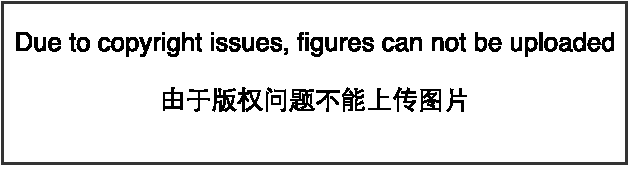
\includegraphics{figure.pdf}}
\else
\centering    
\subfigure{ \label{fig:chap9_Gabor_functions_a}     
\includegraphics[width=0.3\textwidth]{Chapter9/figures/gabor_sinusoid.png}}     
\subfigure{ \label{fig:chap9_Gabor_functions_b}     
\includegraphics[width=0.3\textwidth]{Chapter9/figures/gabor_coordinate_system.png}}
\subfigure{ \label{fig:chap9_Gabor_functions_c}     
\includegraphics[width=0.3\textwidth]{Chapter9/figures/gabor_scale.png}}     
\fi
\caption{Tmp}     
\label{fig:chap9_Gabor_functions}     
\end{figure}

参数$x_0,y_0$和$\tau$定义坐标系。
我们平移和旋转$x$和$y$来得到$x'$和$y'$。
具体地,简单细胞会响应以点$(x_0, y_0)$为中心的图像特征,并且当我们沿着从水平方向旋转$\tau$弧度的线移动时,简单细胞将响应亮度的变化。
 
% -- 357 --
 
作为$x'$和$y'$的函数,函数$w$会响应当我们沿着$x'$移动时的亮度变化。
它有两个重要的因子:一个是Gaussian函数,另一个是余弦函数。

Gaussian因子$ \alpha \exp(-\beta_x x'^2 - \beta_y y'^2)$可以被视为阈值项,用于保证简单细胞仅对接近$x'$和$y'$都为零点处的值响应,换句话说,接近细胞接受域的中心。
尺度因子$\alpha$调整简单细胞响应的总的量级,而$\beta_x$和$\beta_y$控制接受域消退的速度。

余弦因子$ \cos (fx' + \phi)$控制简单细胞如何响应延$x‘$轴的亮度改变。
参数$f$控制余弦的频率,$\phi$控制它的相位偏移。

合在一起,简单细胞的这个卡通视图意味着,简单细胞对在特定位置处、特定方向上、特定空间频率的亮度进行响应。
当图像中的光波与细胞的权重具有相同的相位时,简单细胞是最兴奋的。
这种情况发生在当图像亮时,它的权重为正,而图像暗时,它的权重为负。
当光波与权重完全异相时,简单细胞被抑制——当图像较暗时,它的权重为正;较亮时,它的权重为负。
 
% -- 358 --
 
复杂细胞的卡通视图是它计算包含两个简单细胞响应的2维向量的$L^2$范数:$c(I)=\sqrt{s_0(I)^2 + s_1(I)^2}$。
一个重要的特殊情况是当$s_1$和$s_0$具有除$\phi$ 以外都相同的参数,并且$\phi$被设置为使得$s_1$与$s_0$相位相差四分之一周期时。
在这种情况下,$s_0$和$s_1$形成\firstgls{quadrature_pair}。
当Gaussian重新加权的图像$I(x,y)\exp(-\beta_x x'^2 -\beta_y y^2)$包含具有频率$f$、在方向$\tau$上、接近$(x_0, y_0)$的高振幅正弦波时,用先前方法定义的复杂细胞会响应,并且\textbf{不管该波的相位偏移}。
换句话说,复杂细胞对于图像在方向$\tau$上的微小变换或者翻转图像(用白色代替黑色,反之亦然)具有不变性。

神经科学和机器学习之间最显著的对应关系,是从视觉上比较机器学习模型学得的特征与使用V1得到的特征。
\cite{Olshausen+Field-1996}说明,一个简单的无监督学习算法,稀疏编码,学习的特征具有与简单细胞类似的接收域。
从那时起,我们发现,当应用于自然图像时,极其多样的统计学习算法学习类Gabor函数的特征。这包括大多数深度学习算法,它们在其第一层中学习这些特征。
图\ref{fig:chap9_feature_detectors}给出了一些例子。
因为如此众多不同的学习算法学习边缘检测器,所以很难仅基于学习算法学得的特征,来断定哪一个特定的学习算法是``正确''的大脑模型(虽然,当应用于自然图像时,如果一个算法\emph{不能}学得某种检测器时,它能够作为一种否定标志)。
这些特征是自然图像的统计结构的重要部分,并且可以通过许多不同的统计建模方法来重新获得。
可以参考\citep{hyvarinen-book2009}来获得自然图像统计领域的综述。
% fig 9.19
\begin{figure}
\ifOpenSource
\centerline{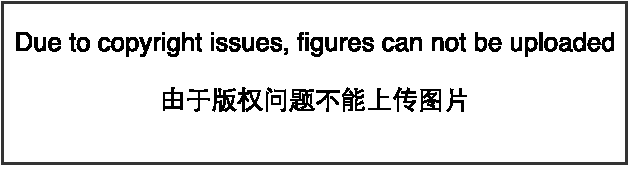
\includegraphics{figure.pdf}}
\else
\centering    
\subfigure{ \label{fig:chap9_feature_detectors_a}     
\includegraphics[width=0.4\textwidth]{Chapter9/figures/maxout_kernels.png}}     
\subfigure{ \label{fig:chap9_feature_detectors_b}     
\centerline{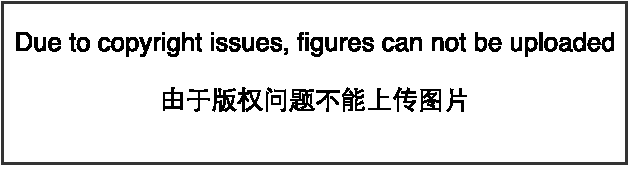
\includegraphics{figure.pdf}}
\includegraphics[width=0.4\textwidth]{Chapter9/figures/s3c_filters.png}}    
\fi
\caption{Tmp}     
\label{fig:chap9_feature_detectors}     
\end{figure}

\section{卷积神经网路与深度学习的历史}
\label{sec:convolutional_networks_and_the_history_of_deep_learning}
 
% -- 359 --
 
\gls{convolutional_network}在深度学习的历史中发挥了重要作用。
它们是将研究大脑获得的深刻理解成功用于机器学习应用的关键例子。
它们也是第一个表现良好的深度模型之一,远远早于任意深度模型被认为是可行的。
\gls{convolutional_network}也是第一个解决重要商业应用的神经网络,并且仍然是当今深度学习商业应用的前沿。
例如,在20世纪90年代,AT\&T的神经网络研究小组开发了一个用于读取支票的\gls{convolutional_network}\citep{chapter-gradient-document-2001}。
到90年代末,NEC部署的这个系统用于读取美国所有支票的10%以上。
后来,微软部署了若干个基于\gls{convolutional_network}的OCR和手写识别系统\citep{simard-03-small}。 
关于\gls{convolutional_network}的这种应用和更现代应用的更多细节,参见第\ref{chap:applications}章。
到2010年以前的更为深入的\gls{convolutional_network}历史可以参见\citep{Lecun_convolutionalnetworks}。

\gls{convolutional_network}也被用来赢得许多比赛。
当前对深度学习的商业兴趣的热度始于\cite{Krizhevsky-2012-small}赢得了ImageNet物体识别挑战,但是\gls{convolutional_network}已经被用于赢得其他机器学习和计算机视觉竞赛了,这些比赛在几年前影响较小。
 
% -- 360 --
 
\gls{convolutional_network}是用反向传播训练的第一个有效的深度网络之一。
现在仍不完全清楚为什么\gls{convolutional_network}在一般的反向传播网络被认为已经失败时反而成功了。
可能简单地归结为\gls{convolutional_network}比全连接网络计算效率更高,因此使用它们运行多个实验并调整它们的实现和超参数更容易。
更大的网络也似乎更容易训练。
利用现代硬件,大型全连接的网络对许多任务也执行得很合理,即使使用过去那些全连接网络被认为不能工作的很好的数据集和当时流行的激活函数时,现在也能执行得很好。
可能神经网络成功的主要阻碍是心理(实践者没有期望神经网络有效,所以他们没有认真努力地使用神经网络)。
无论如何,幸运的是\gls{convolutional_network}在几十年前就表现良好。
在许多方面,它们为余下的深度学习传递火炬,并为一般的神经网络被接收铺平了道路。

\gls{convolutional_network}提供了一种方法来专业化神经网络,以处理具有清楚的网格结构拓扑的数据,以及将这样的模型放大到非常大的尺寸。 
这种方法在二维图像拓扑上是最成功的。
为了处理一维序列数据,我们接下来转向神经网络框架的另一种强大的专业化:循环神经网络。

 
% -- 361 --
 










